\chapter{Semi-Unsupervised Approach}

Unsupervised methods, consider a human fall as an event that deviate from normality and they are based on one-class classifiers. The main advantage of an unsupervised methods for fall detection is that it can works without knowing any examples related the the class of interest, i.e. the human fall. As aforementioned, this should be the perfect way to go in an application like this, where what we are interested in is very difficult to retrieve or we only have very few data available, but the principal weakness of an unsupervised system is that certain events deviate from normality as the human fall (e.g., the fall of an object), thus they may produce false alarms.
In this Chapter, two types of methods are described: in \secref{sec:user_aided_cin} a OCSVM used-ided method is exposed, while \secref{sec:siamese_few_shot} present an approach based on Siamese neural network for one-shot learning, both of them assessed with samples related to R0 room of the employed dataset \secref{sec:dataset}. An extension of the Siamese approach is presented in \secref{sec:siamese_few_shot} where the entire dataset presented in \secref{sec:dataset} has been used.




\section{A Combined One-Class SVM and Template Matching Approach for User-Aided Human Fall Detection}
\label{sec:user_aided_cin}

The approach proposed here, is the extension of the one presented in \secref{sec:ocsvm_approach} thus, consists of a combined One-Class Support Vector Machine (OCSVM) based method and template-matching classifier that operate in cascade. The template-matching classifier operates in a user-aided supervised manner and it is employed to reduce such errors by using a set of templates that represent these events. Templates are identified by the user that marks the occurrence of a false positive instead of a true human fall event. 
As shown in the previous section, ``unsupervised methods'' are able to overcome the need of manual tuning of ``analytical methods'' and the necessity of a large labelled dataset of ``supervised methods''. In ``unsupervised methods'', falls are discriminated from non-falls based on a model of ``normality'' constructed from a large amount of non-fall events. However, certain events differ from the ``normality'' as human falls, and they may induce the classifier to produce false alarms. As an example, \figref{fig:time_ha} and \figref{fig:spec_ha} show respectively the waveform and the spectrogram of a segment of ``normal'' human activity (footsteps and speech) \figref{fig:time_hf} and \figref{fig:spec_hf} show the waveform and the spectrogram of a segment of human fall, and \figref{fig:time_bf} and \figref{fig:spec_bf} the waveform and the spectrogram of a book fall. The figures show clearly that both falls signals differ significantly from the human activity one, thus a classifier may be induced to consider the fall of a book as the fall of a person.

\begin{figure}[htbp!]
	\centering
	\begin{subfigure}[t]{0.5\columnwidth}
		\centering
		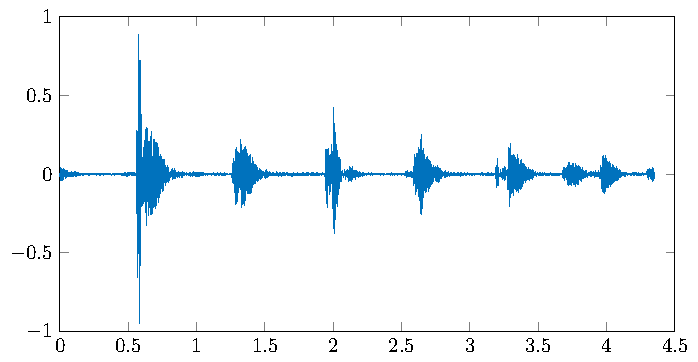
\includegraphics[width=0.9\textwidth]{img/cin/ha_time_.pdf}
		\caption{Normal human activity signal in the time domain.}\label{fig:time_ha}
	\end{subfigure}%
	\begin{subfigure}[t]{0.5\columnwidth}
		\centering
		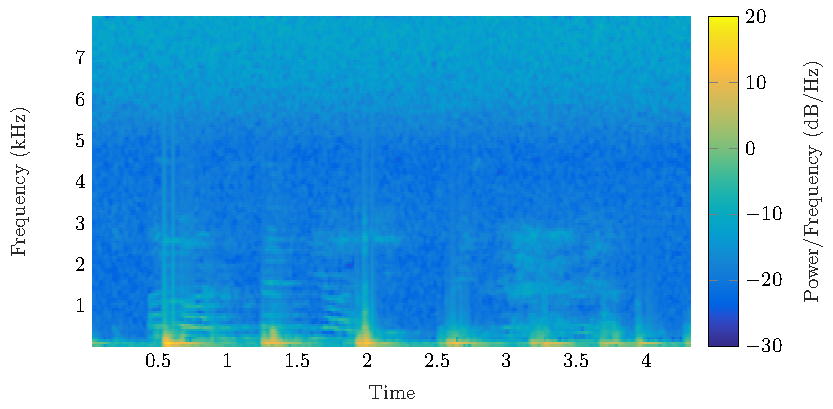
\includegraphics[width=\textwidth]{img/cin/ha_freq_.pdf}
		\caption{Normal human activity signal in the frequency domain.}\label{fig:spec_ha}
	\end{subfigure}
	
	\begin{subfigure}[t]{0.5\columnwidth}
		\centering
		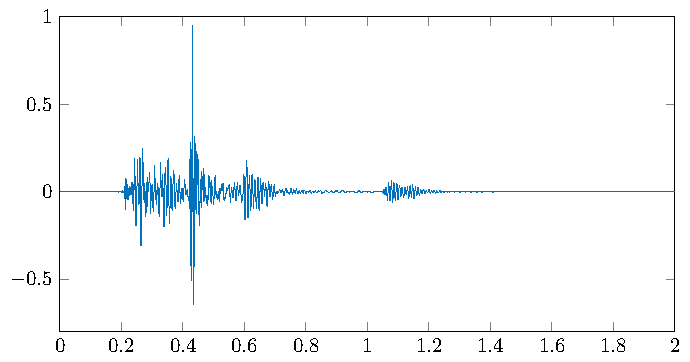
\includegraphics[width=0.9\textwidth]{img/cin/rndy_time_.pdf}
		\caption{Human fall signal in the time domain.}\label{fig:time_hf}
	\end{subfigure}%
	\begin{subfigure}[t]{0.5\columnwidth}
		\centering
		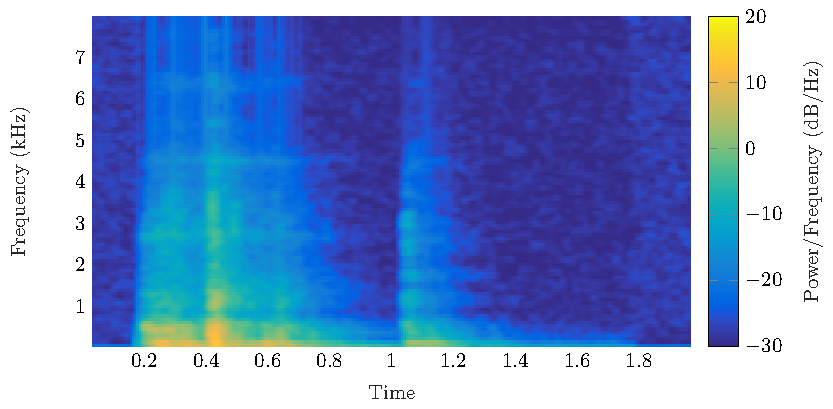
\includegraphics[width=\textwidth]{img/cin/rndy_freq_.pdf}
		\caption{Human fall signal in the frequency domain.}\label{fig:spec_hf}
	\end{subfigure}
	
	\begin{subfigure}[t]{0.5\columnwidth}
		\centering
		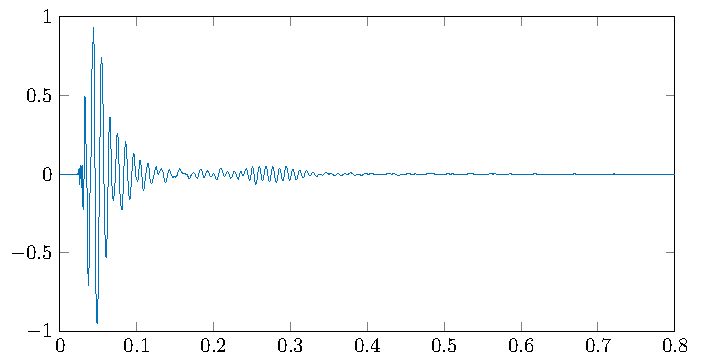
\includegraphics[width=0.9\textwidth]{img/cin/book_time_.pdf}
		\caption{Book fall signal in the time domain.}\label{fig:time_bf}
	\end{subfigure}%
	\begin{subfigure}[t]{0.5\columnwidth}
		\centering
		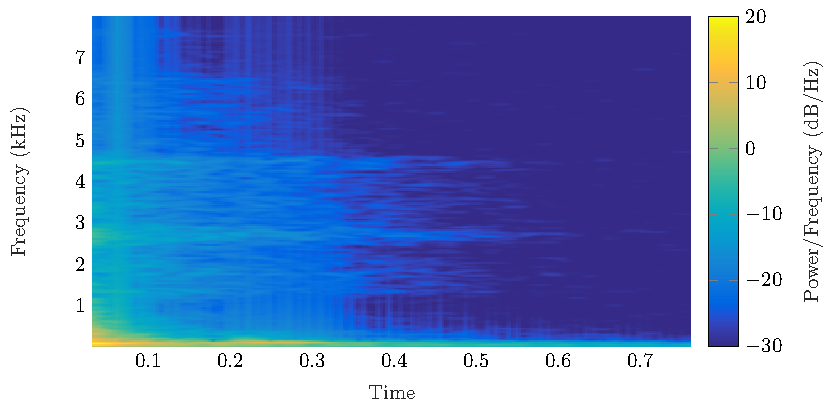
\includegraphics[width=\textwidth]{img/cin/book_freq_.pdf}
		\caption{Book fall signal in the frequency domain.}\label{fig:spec_bf}
	\end{subfigure}
	\caption{Time domain (on the left) and frequency domain (on the right) representation of a normal human activity signal (a-b), human fall signal (c-d), and book fall signal (e-f).}\label{fig:waveforms}
\end{figure}

The algorithm proposed in this paper reduces the problem by employing a multi-stage classification approach that combines a one-class classifier based on OCSVM with a template-matching stage. The OCSVM is trained unsupervisedly on a large corpus containing sounds that represent the ``normality''. On the contrary, the template-matching stage employs a set of templates represented by a small number of feature vectors marked as false alarm by the user. Thus, robustness against possible false alarms is achieved by using only few examples of false positive classes without the need of multiple sensors. An additional advantage with respect to the state of the art is that the proposed approach is able to evolve and improve after its initial training, since the template set can be augmented as non-falls events are detected.

\subsection{Proposed approach}
The proposed approach is composed of three stages \figref{fig:overall_ocsvm_user_aided}: the first (``Feature Extraction'') extracts MFCCs from the input audio signal and then GMSs to describe the entire audio segment. The second stage (``Abnormal Event Detection'') consists of a One-Class SVM classifier that discriminates between normal and abnormal sounds. Up to the authors' knowledge, OCSVM together with GMSs have never been jointly used for acoustic fall detection.  The third stage represents the innovative contribution of this paper for reducing false alarms in unsupervised approaches: it consists of a ``Template-Matching'' block that refines the output of the OCSVM and classifies the input data as fall or non-fall. The OCSVM is trained unsupervisedly on a large dataset of everyday sounds with the objective of discriminating normal from abnormal sounds. As aforementioned, the basic assumption is that the acoustic events related to human falls are ``rare'' respect to sounds normally occurring inside a home. The template-matching stage, on the other side, requires a set of ``template'' instances that represent rare events that can be confused with a fall. Referring to \figref{fig:overall_ocsvm_user_aided}, the ``Template-Matching'' stage is composed of a set of ``Templates'', a block that calculates the distance between the input GMS and the templates (``Euclidean Distance Calculation''), and a ``Decision'' block the decides whether the event is a fall or a non-fall by evaluating the magnitude of the distance.  The rationale here is that certain acoustic events are as abnormal as falls and confuse the OCSVM: the template-matching stage reduces false positives by using a set of examples related to the most confusing classes. In this work, the algorithm is ``user-aided'', i.e., templates are indicated by the user each time the OCSVM produces a false positive. This is shown in \figref{fig:overall_ocsvm_user_aided} with the person silhouette near the block that decides whether a detected fall is a false positive or not (``False Positive?''). In general, however, it is possible to create the templates set a-priori by recording several instances of possible false alarms events. Although rare, false alarm events (e.g., falls of objects) are certainly easier to reproduce in laboratory respect to human falls. The remainder of this sections describes the overall approach in details, starting from the acoustic sensor employed for capturing falls sounds, the feature extraction stage, and the combined OCSVM/template-matching stages.

\begin{figure}[t]
	\centering
	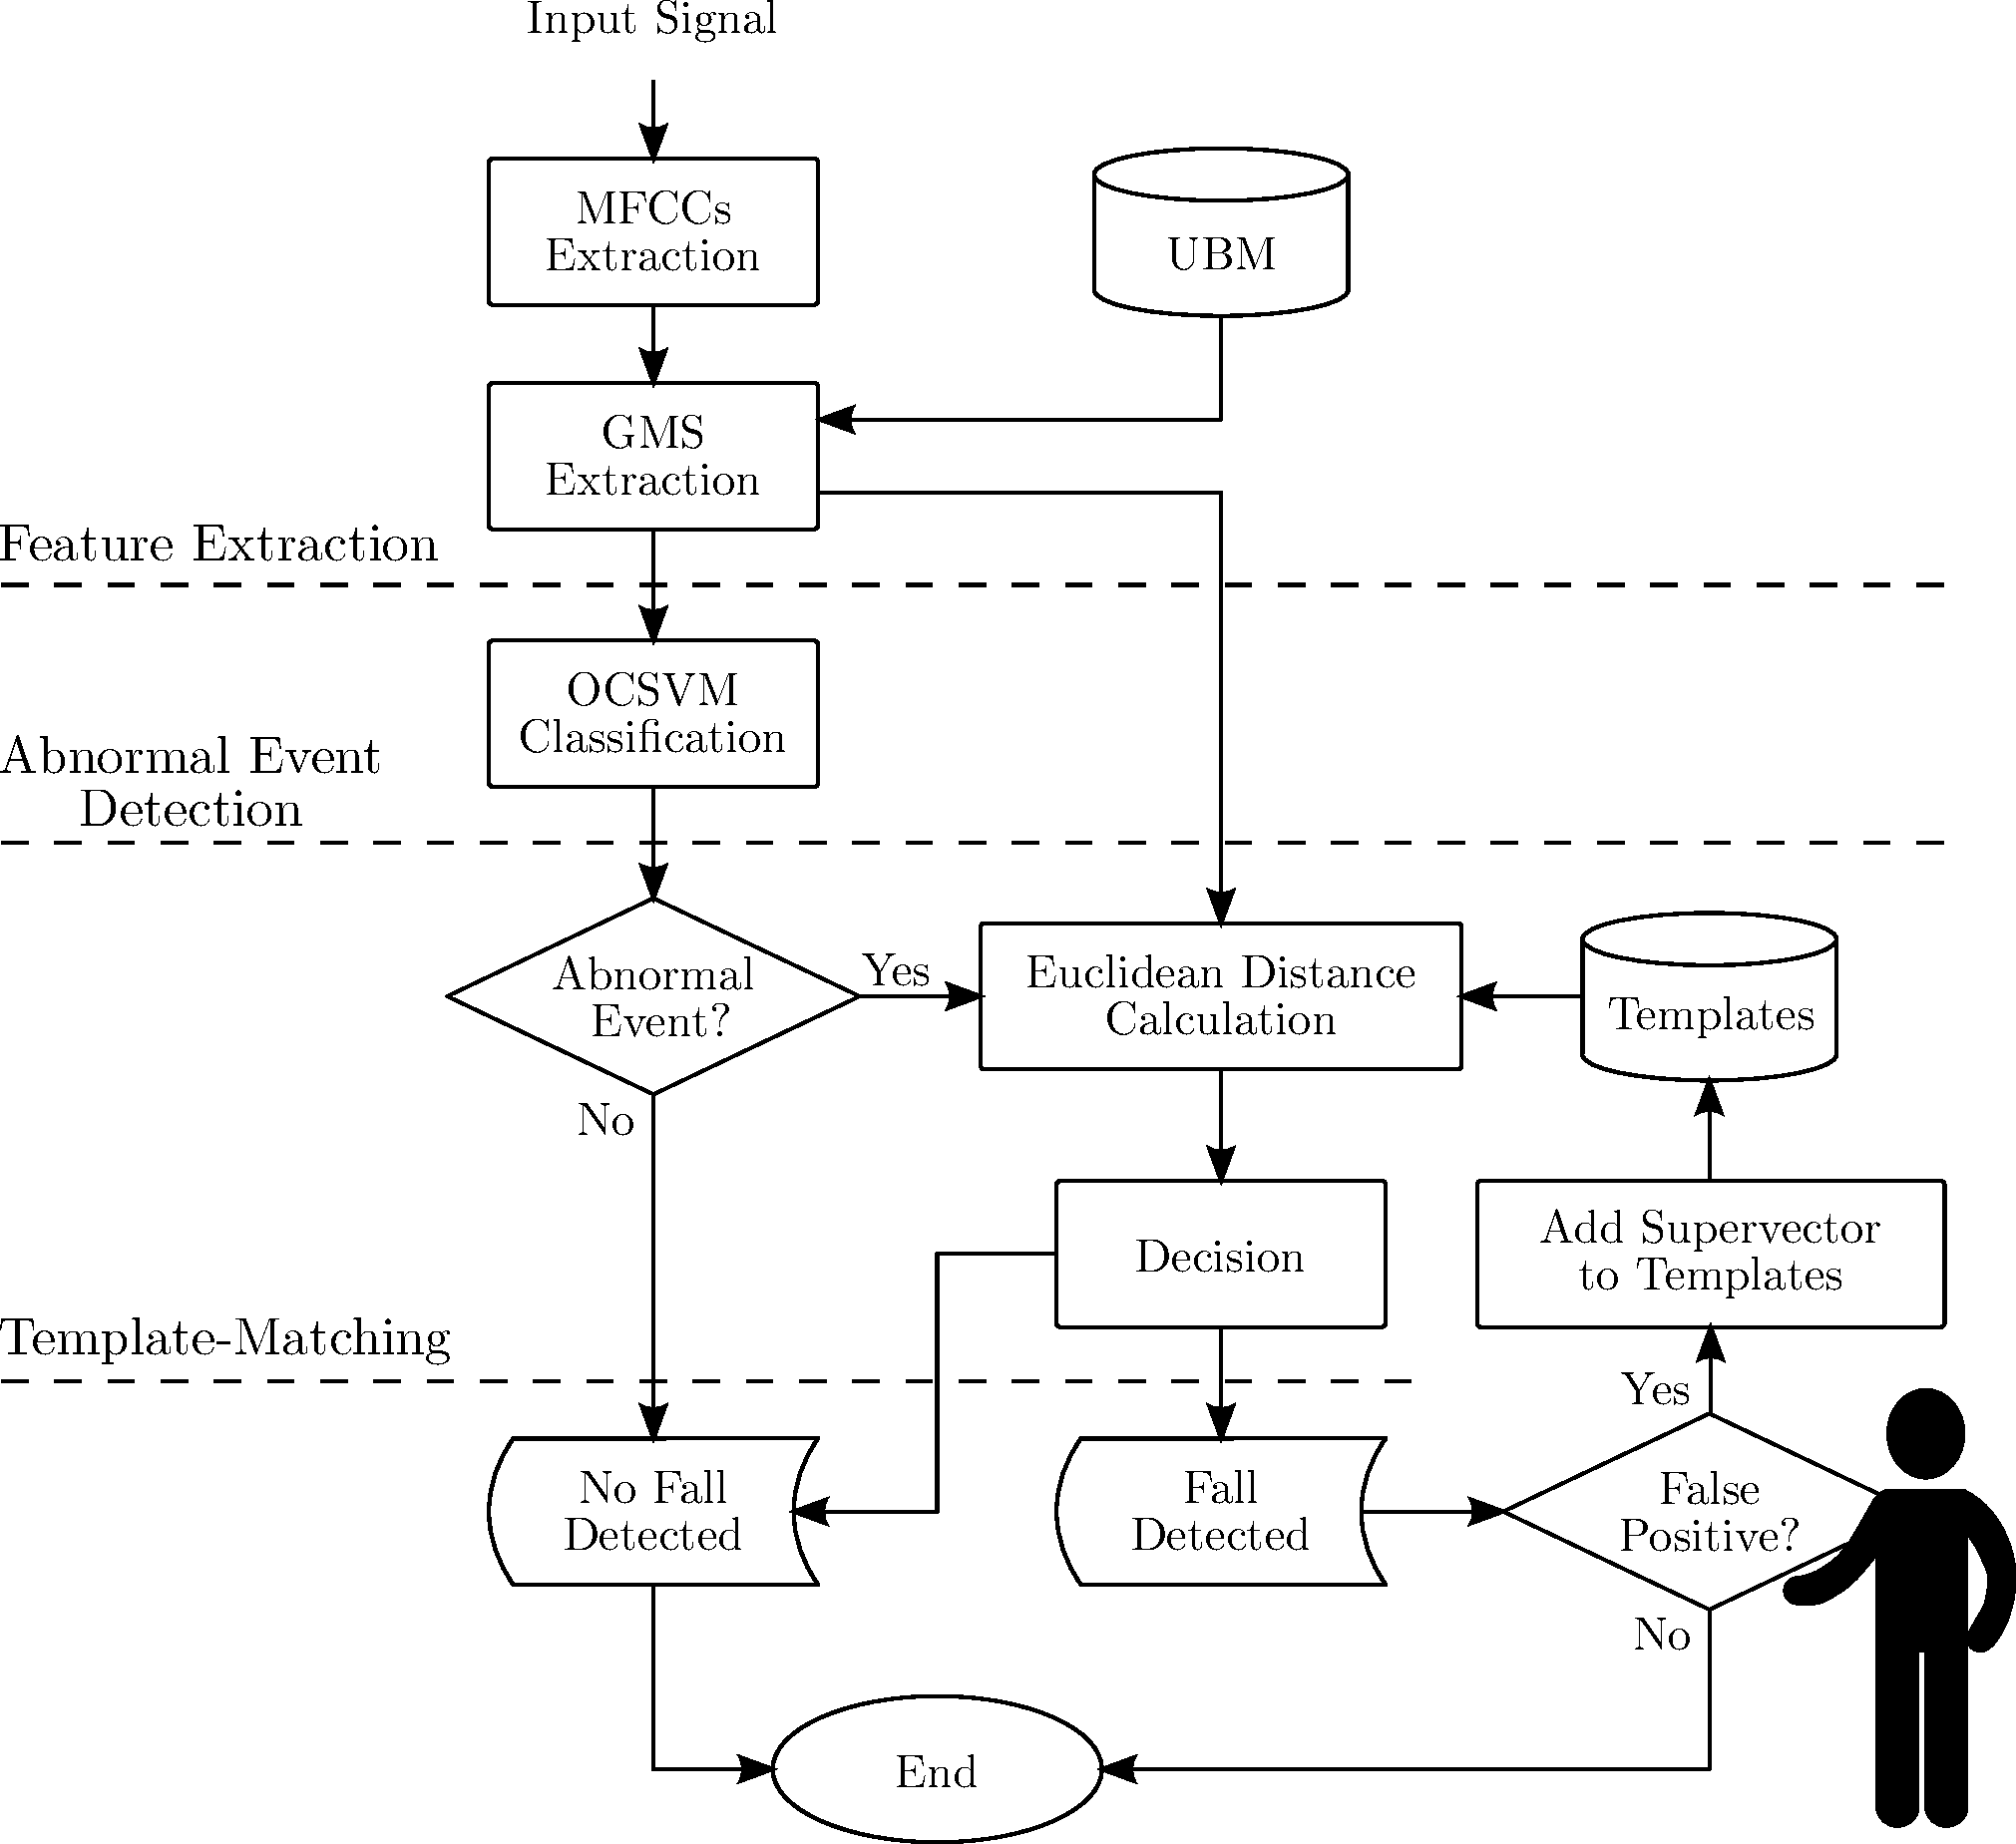
\includegraphics[width=0.95\columnwidth]{img/cin/approccioComplessivo.pdf}
	\caption{The block scheme of the proposed approach.}\label{fig:overall_ocsvm_user_aided}
\end{figure}

\subsection{Dataset}

The dataset employed in this method is reported in \tableref{tab:trainComposition} of a previous section

\section{Few-shot Siamese Neural Networks employing Audio features
for Human-Fall Detection}
\label{sec:siamese_few_shot}
\section{Audio Metric Learning by using Siamese Autoencoders
for One-Shot Human Fall Detection}
\label{sec:siamese_one_shot}